%%=============================================================================
%% Performantietest
%%=============================================================================

\chapter{Performantie test}
\label{ch:performantietest}

In dit hoofdstuk worden de resultaten besproken van de uitgevoerde performantietests.

De performantie van beide systemen werd op twee manieren getest:
Eerst werd de benodigde tijd gemeten voor het uitvoeren van het 'vagrant up'-commando. Dit commando installeerde en configureerde het besturingssysteem, de applicaties en de containers vanaf nul.

Vervolgens werd de benodigde tijd gemeten bij het uitvoeren van het 'vagrant provision'-commando. Hierbij waren het besturingssysteem en de applicaties al geïnstalleerd en geconfigureerd, en moesten alleen de containers nog tot stand gebracht worden. Om de internetsnelheid als factor te schrappen, waren de Docker Images ook al gedownload.

Daarnaast werd 'time' als prefix aan het commando toegevoegd. Hierdoor werd de benodigde uitvoeringstijd op het einde van de commando's getoond.

Vervolgens werden beide commando's vijftien keer uitgevoerd op beide opstellingen. Hierdoor werd de invloed van outliers verminderd. Outliers zijn observatiepunten die ver van andere punten verwijderd liggen.

Ten slotte werden deze resultaten genoteerd in een tabel in Rstudio, zodat deze resultaten konden worden gebruikt om het gemiddelde, de variantie en standaarddeviatie te berekenen, alsook voor het genereren van een scatterplot en boxplot.

\section{CentOS 7.4}

\subsection{Performantie installatie}
Hieronder kan men de eerste resultaten zien van het 'time vagrant up'-commando voor de CentOS-opstelling.

%table
\begin{table}
	\centering
	\begin{tabular}{lllllllllllllll}
		\hline
		Meting 1 & Meting 2 & Meting 3 & Meting 4 & Meting 5 & Meting 6 & Meting 7 & Meting 8 & Meting 9 & Meting 10 & Meting 11 & Meting 12 & Meting 13 & Meting 14 & Meting 15 \\
		\hline
		5m0.840s & 5m7.846s & Meting 3 & Meting 4 & Meting 5 & 5m4.108s & 4m36.605s & 4m17.360s & 4m40.993s & 4m27.195s & 4m15.713s & 4m9.928s & 4m30.109s & 4m31.078s & 4m44.484s \\
		\hline
	\end{tabular}
\caption{De resultaten van 'time vagrant up' voor de CentOS-opstelling.}
\label{tab:timevagrantupcentos}
\end{table}

%% plot

\begin{figure}
	\centering
	\caption{De scatterplot voor de resulaten van 'time vagrant up' voor de CentOS-opstelling}
	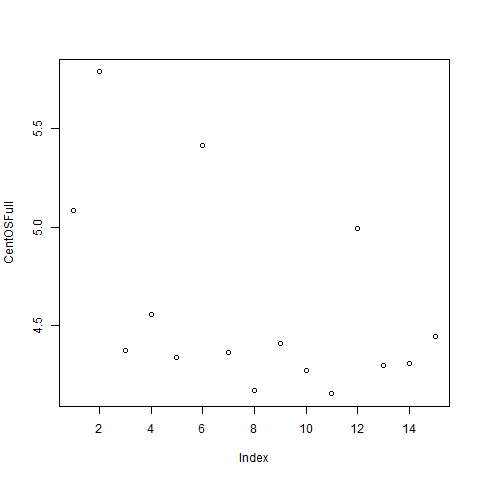
\includegraphics[scale=0.5]{img/centosfullplot.png}
	\label{fig:centosupplot}
\end{figure}

%% boxplot
\begin{figure}
	\centering
	\caption{De boxplot voor de resulaten van 'time vagrant up' voor de CentOS-opstelling}
	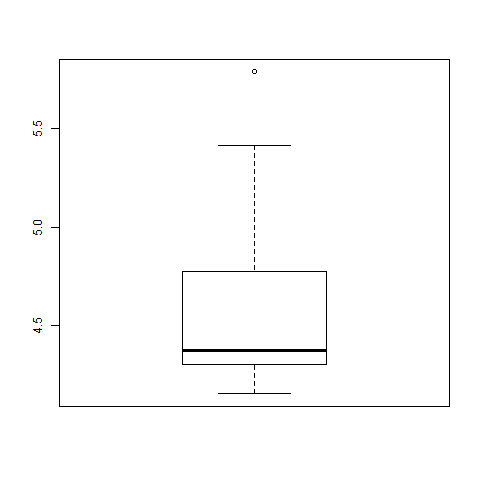
\includegraphics[scale=0.5]{img/centosfullboxplot.png}
	\label{fig:centosupboxplot}
\end{figure}

%% gemiddelde, variantie en standaarddeviatie
\[\mu = 4.59897 \sigma^2 = 0.2386372 \sigma = 0.488505\]

De gemiddelde benodigde tijd voor het commando bij de CentOS-opstelling was laag en vrijwel stabiel, met slechts enkele outliers. De reden voor deze outliers was omdat het ophalen van een Docker Image gevoelig is aan slechtere internetverbindingen. Dit was de grootste bottleneck voor deze opstellingen. De impact hiervan op de installatie was in dit geval groot, zoals te zien is aan de hoge variatie en de standaarddeviatie. Maar, over het algemeen is de performantie van de CentOS-opstelling wel goed te noemen.

\subsection{Performantie containers}
Hieronder kan men de resultaten zien voor elke keer dat het 'time vagrant provision'-commando werd uitgevoerd op de CentOS-opstelling, maar dan deze keer uitgedrukt in seconden. Bij deze resultaten moest het Operating System niet meer geïnstalleerd worden en ook de Docker Image moest niet meer gedownload worden. Er werd alleen gekeken hoeveel tijd de Docker Daemon nodig had om de orders te interpreteren en de container op te stellen.

%table
\begin{table}
	\centering
	\begin{tabular}{lllllllllllllll}
		\hline
		Meting 1 & Meting 2 & Meting 3 & Meting 4 & Meting 5 & Meting 6 & Meting 7 & Meting 8 & Meting 9 & Meting 10 & Meting 11 & Meting 12 & Meting 13 & Meting 14 & Meting 15 \\
		\hline
		7.062s & 5.839s & 5.804s & 6.000s & 5.733s & 6.415s & 5.911s & 5.844s & 5.856s & 5.854s & 5.861s & 5.850s & 5.898s & 5.802s & 5.856s \\
		\hline
	\end{tabular}
	\caption{De resultaten van 'time vagrant provision' voor de CentOS-opstelling.}
	\label{tab:timevagrantprovisioncentos}
\end{table}

%% plot
\begin{figure}
	\centering
	\caption{De scatterplot voor de resulaten van 'time vagrant provision' voor de CentOS-opstelling}
	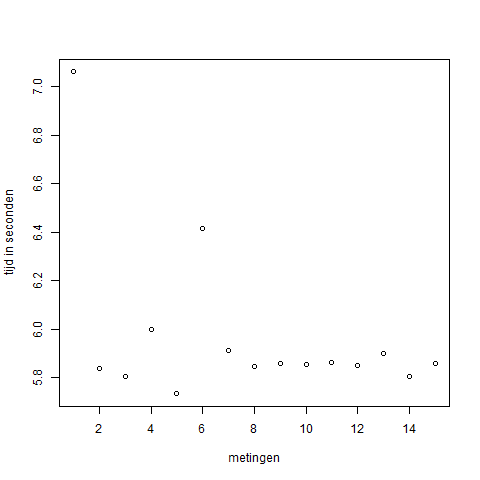
\includegraphics[scale=0.5]{img/centosplotprovision.png}
	\label{fig:centosprovisionplot}
\end{figure}

%% boxplot
\begin{figure}
	\centering
	\caption{De boxplot voor de resulaten van 'time vagrant provision' voor de CentOS-opstelling}
	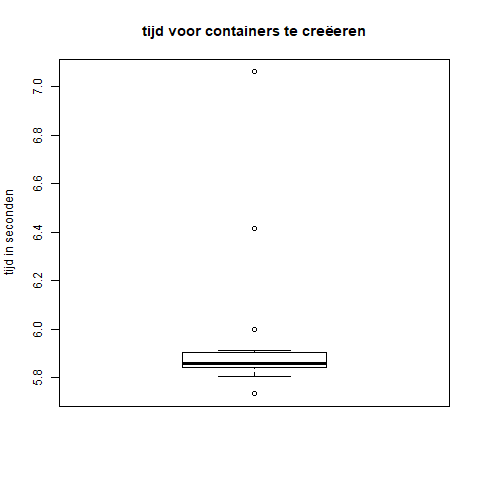
\includegraphics[scale=0.5]{img/centosboxplotprovision.png}
	\label{fig:centosprovisionboxplot}
\end{figure}

%% gemiddelde, variantie en standaarddeviatie
\[\mu = 5.972333 \sigma^2 = 0.1150491 \sigma = 0.3391889\]

De installatie van enkel de container verliep vlot, met een stabielere gemiddelde tijd en een kleinere variantie en standaarddeviatie. Dit kwam doordat de applicaties en Docker Images niet meer moesten worden gedownload. Hierdoor lagen de tijden veel lager en was er geen invloed meer van de bottleneck.

\section{Windows Server 2016}
\subsection{Performantie installatie}
Hieronder kan men de resultaten zien van 'time vagrant up' voor de Windows-opstelling.

%table
\begin{table}
	\centering
	\begin{tabular}{lllllllllllllll}
		\hline
		Meting 1 & Meting 2 & Meting 3 & Meting 4 & Meting 5 & Meting 6 & Meting 7 & Meting 8 & Meting 9 & Meting 10 & Meting 11 & Meting 12 & Meting 13 & Meting 14 & Meting 15 \\
		\hline
		51m16.108s & 54m17.881s & 50m9.325s & 48m57,389s & 40m31.108s & 47m27.296s & 46m56.752s & 50m29.209s & 51m36,846s & 50m20,653s & 48m48.415s & 53m23.226s & 48m32.114s & 47m20.920s & 49m7.544s \\
		\hline
	\end{tabular}
	\caption{De resultaten van 'time vagrant up' voor de Windows-opstelling.}
	\label{tab:timevagrantupwindows}
\end{table}

%% plot
\begin{figure}
	\centering
	\caption{De scatterplot voor de resulaten van 'time vagrant up' voor de Windows-opstelling}
	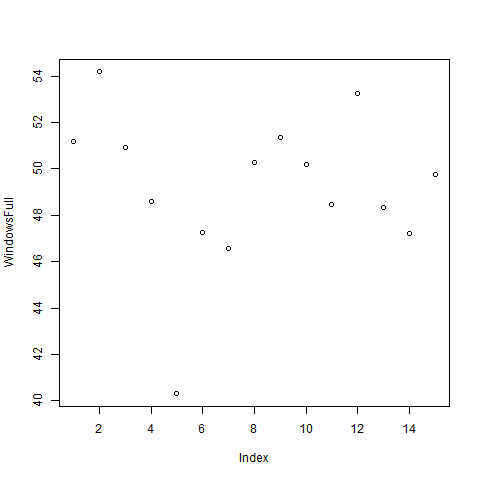
\includegraphics[scale=0.5]{img/windowsplotfull.png}
	\label{fig:windowsupplot}
\end{figure}

%% boxplot
\begin{figure}
	\centering
	\caption{De boxplot voor de resulaten van 'time vagrant up' voor de Windows-opstelling}
	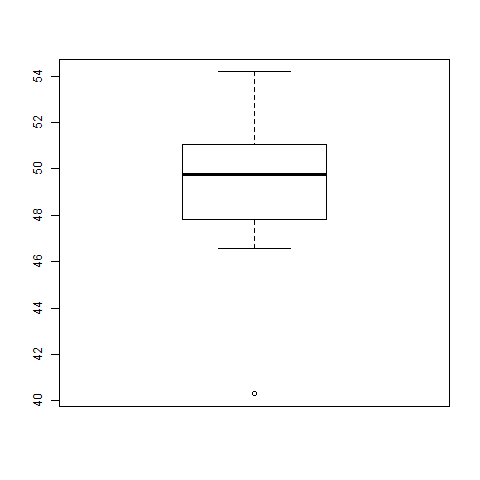
\includegraphics[scale=0.5]{img/windowsboxplotfull.png}
	\label{fig:windowsupboxplot}
\end{figure}

%% gemiddelde, variantie en standaarddeviatie
\[\mu = 49.19089 \sigma^2 = 10.74354 \sigma = 3.277733\]

De installatie van de Windows-opstelling duurde gemiddeld 10 keer langer dan de centOS-opstelling. De gemiddelde tijd voor een volledige installatie bedroeg immers 45 minuten. De variantie en standaarddeviatie waren wel klein. Hier zijn verschillende redenen voor:

\begin{itemize}[noitemsep]
	\item Installatie Windows OS
\end{itemize}

Om te beginnen duurde de installatie van het besturingssysteem langer omdat er een GUI gebruikt werd. Als men de Windows Server Core zou gebruiken, zou de performantie al sterk verbeteren, maar dan kon men geen Docker CE for Windows installeren. Windows Server Nano was helaas ook geen optie, omdat deze helemaal niet ondersteund werd door Docker for Windows, zelfs niet voor Docker EE. Ten slotte hoefde CentOS ook niet heropgestart te worden na de installatie van Docker. \autocite{xlegalles2017}

\begin{itemize}[noitemsep]
	\item Microsoft SQL server container
\end{itemize}

De MSSQL server container voor Windows was meer dan 10 keer zo groot als de Linux variant, meer specifiek: 6GBs tegenover 479MBs. Hierdoor was de installatie een groot deel van de tijd bezig met het downloaden van deze Docker Image. \autocite{Moon2017}

\subsection{Performantie applicatie}
Hieronder kan men de resultaten zien van 'time vagrant provision' voor de Windows-opstelling van alleen de benodigde tijd om de containers te installeren.

%table
\begin{table}
	\centering
	\begin{tabular}{lllllllllllllll}
		\hline
		Meting 1 & Meting 2 & Meting 3 & Meting 4 & Meting 5 & Meting 6 & Meting 7 & Meting 8 & Meting 9 & Meting 10 & Meting 11 & Meting 12 & Meting 13 & Meting 14 & Meting 15 \\
		\hline
		21.771s & 15.876s & 15.573s & 17.115s & 16.873s & 16.335s & 15.068s & 19.243s & 17.221s & 16.437s & 16.539s & 17.440s & 15.372s & 16.477s & 15.675s \\
		\hline
	\end{tabular}
	\caption{De resultaten van 'time vagrant provision' voor de Windows-opstelling.}
	\label{tab:timevagrantprovisionwindows}
\end{table}

%% plot
\begin{figure}
	\centering
	\caption{De scatterplot voor de resulaten van 'time vagrant provision' voor de Windows-opstelling}
	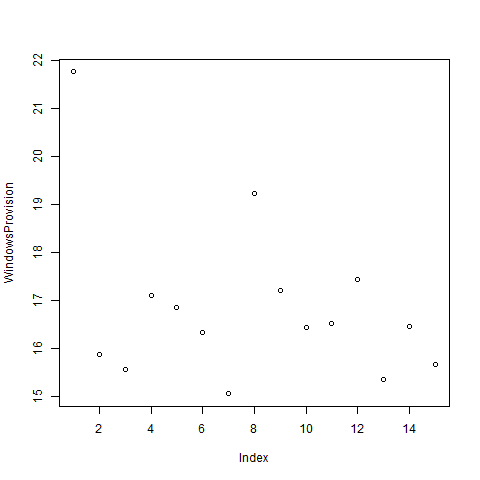
\includegraphics[scale=0.5]{img/WindowsProvisionplot.png}
	\label{fig:windowsprovisionplot}
\end{figure}

%% boxplot
\begin{figure}
	\centering
	\caption{De boxplot voor de resulaten van 'time vagrant provision' voor de Windows-opstelling}
	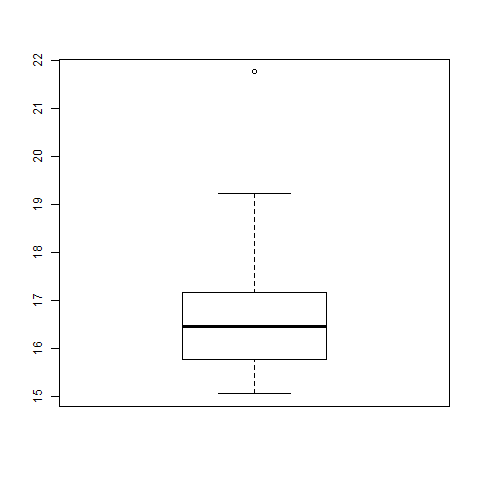
\includegraphics[scale=0.5]{img/WindowsProvisionboxplot.png}
	\label{fig:windowsprovisionboxplot}
\end{figure}

%% gemiddelde, variantie en standaarddeviatie
\[\mu = 16.86767 \sigma^2 = 1.70055 \sigma = 2.89187\]

Hier waren de resultaten al iets meer gelijkaardig aan de CentOS-opstelling, doordat de Windows-opstelling nu geen tijd meer verloor aan de installatie van een GUI, aan heropstarten of aan het downloaden van grotere Docker Images. De voornaamste reden waarom de uitvoeringstijd voor de containers tot drie keer groter was, kwam door de grote van de MSSQL server image. Daarnaast zijn Hyper-V Containers inherent ook groter.

\section{Conclusie}
Op elk vlak scoort CentOS beter voor deze test dan Windows. Zoals opgesomd waren hier verschillende redenen voor. Maar, de meeste van deze redenen kunnen en zullen weggewerkt worden door Microsoft en Docker.